\documentclass{report}
\usepackage[utf8]{inputenc}
\usepackage[russian]{babel}
\usepackage{amsmath}
\usepackage{amsfonts}
\usepackage{amssymb}
\usepackage[dvips]{graphicx}
%\usepackage{{noiseimages/}}

\title{GPS-raw data project}
\author{DSPLab IT-6 mguPI}
\date{2009}

\begin{document}

\maketitle

\chapter{Расчет времен передачи и доступа к элементам платы}
\section{SRAM и GPS}

Частота работы платы 50Mhz=20ns. Длительность цикла чтения/записи из/в SRAM для чипа M5M5V208FP-85L 85ns\\

Цикл операции записи в SRAM:
\begin{tabbing}
Название цикла\qquad\=Обозначение\qquad\=Время\qquad\=Тактов кварца\qquad\=Реальное время\\
\\
выставить адрес \> tsu(A) \> 0ns \> 0 \> 0ns \\
выставить WE/OE \> tdis(W) \> 30ns \> 2 \> 40ns \\
выставить данные \> tsu(D) \> 35ns \> 2 \> 40ns \\
снять WE/OE \> ten(W) \> 5ns \> 1 \> 20ns \\
\\
Итого \> \> 5 \> 100ns \\
\end{tabbing}

Цикл операции чтения из SRAM:
\begin{tabbing}
Название цикла\qquad\=Обозначение\qquad\=Время\qquad\=Тактов кварца\qquad\=Реальное время\\
\\
выставить адрес \> ta(A) \> 85ns \> 5 \> 100ns \\
\\
Итого \> \> 5 \> 100ns \\
\end{tabbing}

GPS микросхема MAX2769 работает на частоте 16.368Mhz. Каждый такт выдается 4 бита: 2-синфазных и 2 квадратурных. Реальная частота
8.184Mhz (для получения 1 байта = 8 бит данных). В пересчете на время получаем:

\begin{equation}
8.184Mhz = 122.18964ns = 1byte 
\end{equation}

\begin{equation}
2^{18} = 256Kbytes\quad\mbox{ (ширина адресной шины в SRAM) }
\end{equation}

Время заполнения памяти (256 Кбайт):

\begin{equation}
122.18964 * 2^{18} = 0.0320313sec 
\end{equation}

Скорость выдачи данных чипом GPS:
\begin{equation}
122.18964sec * 1Mb = 0.1281251\quad Mb/sec\quad\mbox{ (1Мб вычитывается за 0.13 секунды) }
\end{equation}

\begin{equation}
\frac{1Mb}{0.1281251sec} = 7.8\quad Mb/sec
\end{equation}

\section{RS-232}

\begin{equation}
\frac{2^{18}}{
	(\cfrac{115200bits/sec}{8 bits})}   = 18.2 sec\quad\mbox{(время передачи 256Кб данных)}
\end{equation}

\section{Архитектура}
Архитектура hardware части включает в себя несколько блоков: RS-232 порт, микросхему GPS, арбитр управления и контроллер памяти.
\begin{figure}[h]
\center{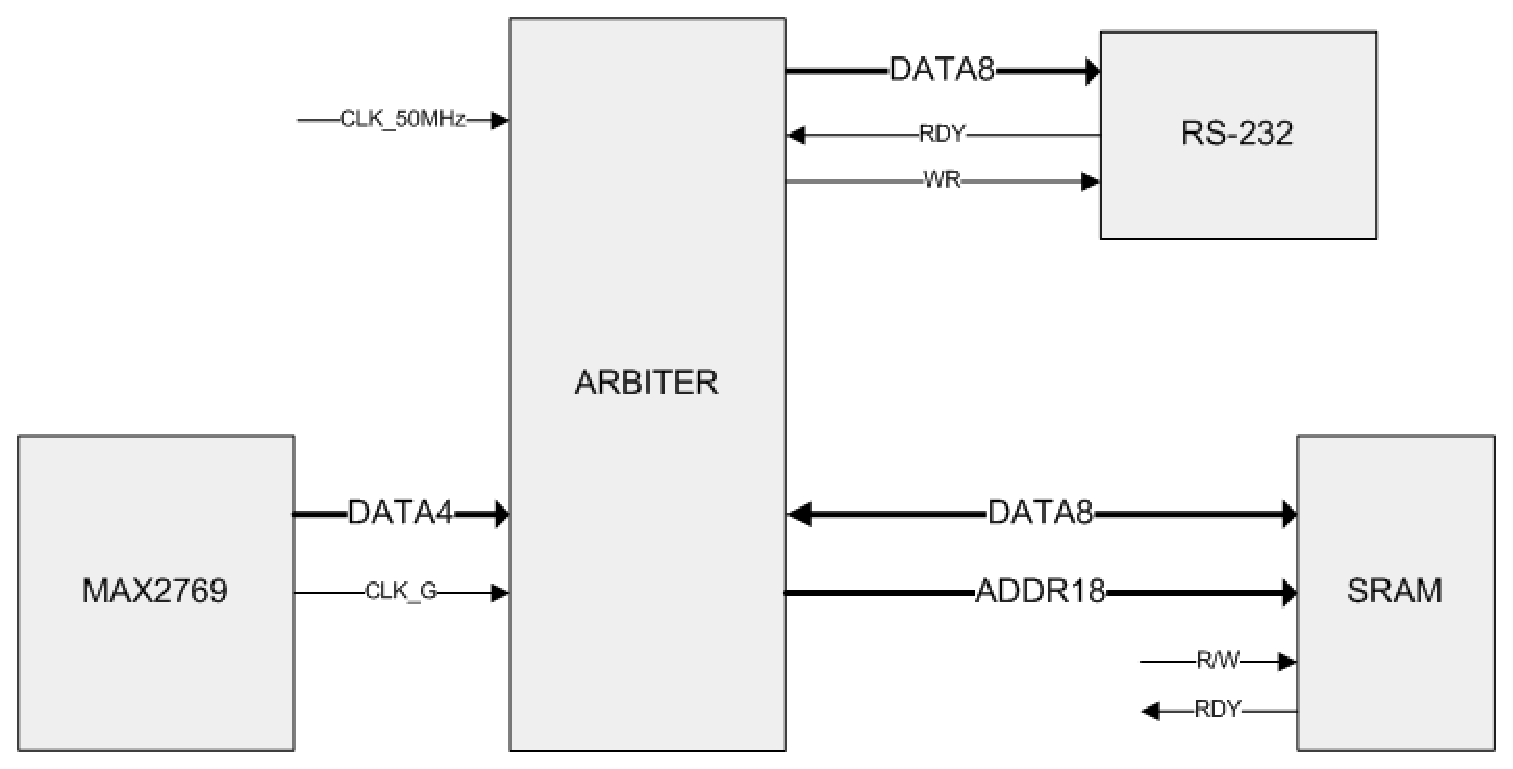
\includegraphics[width=1\linewidth]{./pics/hd_arch.eps}}
\caption{Архитектура hardware-части}
\end{figure}

\end{document}
